% Relatorio da terceira entrega - formato aproximado do modelo SBC
\documentclass[12pt,a4paper]{article}
\usepackage[T1]{fontenc}
\usepackage[utf8]{inputenc}
\usepackage[brazil]{babel}
\usepackage{times}
\usepackage[top=3.5cm,bottom=2.5cm,left=3cm,right=3cm]{geometry}
\usepackage{graphicx}
\usepackage{booktabs}
\usepackage{tabularx}
\usepackage{amsmath}
\usepackage{caption}
\usepackage{url}
\usepackage[hidelinks]{hyperref}
\usepackage{titlesec}
\usepackage{enumitem}

\captionsetup{font={small,bf},labelsep=period}
\titleformat{\section}{\fontsize{13}{15}\bfseries}{\thesection.}{0.5em}{}
\titleformat{\subsection}{\fontsize{12}{14}\bfseries}{\thesubsection.}{0.5em}{}
\titlespacing*{\section}{0pt}{12pt}{6pt}
\titlespacing*{\subsection}{0pt}{12pt}{6pt}
\setlength{\parindent}{1.27cm}
\setlength{\parskip}{6pt}
\setlist{itemsep=1pt,topsep=2pt}
\pagestyle{plain}

\begin{document}

\begin{center}
{\fontsize{16}{20}\bfseries Servidor HTTP/1.1 com Qualidade de Serviço\\ em C com Pthreads: segunda versão\par}
\vspace{12pt}
{\bfseries Giovana Piazza, Luis Felipe Maccalli, Vitor Moreira\par}
\vspace{6pt}
Universidade Federal do Pampa (Unipampa)\\
Fundamentos e Avaliação de Redes de Computadores --- 2026/2
\end{center}

\vspace{6pt}
\begin{list}{}{\leftmargin=0.8cm\rightmargin=0.8cm}\item\itshape
\textbf{\upshape Resumo.} Este relatório apresenta a segunda versão do servidor HTTP
desenvolvido em C com sockets TCP e Pthreads. Sobre a base concorrente e persistente da
primeira versão, foram incorporados mecanismos de Qualidade de Serviço: taxa máxima por
endereço IP lida de um arquivo, taxa padrão de 1000\,kbps, envio controlado de objetos
não HTML, divisão da taxa entre conexões do mesmo IP, controle de admissão pela vazão
máxima do servidor e um painel em tempo real com estimativas de RTT, atraso e banda. Os
experimentos com quatro endereços de origem mostraram vazões no máximo 0,5\% acima das
taxas configuradas e recusa correta de um cliente que excederia a capacidade.
\end{list}

%=====================================================================
\section{Introdução}

O trabalho prático da disciplina propõe o desenvolvimento, em ambiente Linux, de um
servidor HTTP em linguagem C com Pthreads, em versões incrementais. A primeira versão,
apresentada na segunda entrega, atendia clientes concorrentes com conexões persistentes
HTTP/1.1. A segunda versão, objeto desta terceira entrega, deve incorporar os mecanismos de
Qualidade de Serviço (QoS) definidos no enunciado~\cite{spec}:

\begin{itemize}
  \item enviar objetos, exceto o arquivo HTML, com taxa controlada conforme o IP de origem,
  definida em um arquivo auxiliar; IPs não cadastrados devem ser atendidos a 1000\,kbps, se viável;
  \item apresentar visualmente, em tempo real, os clientes atendidos, com estimativa de
  atraso fim-a-fim e largura de banda baseada no RTT, obtido pelo intervalo entre a
  requisição do HTML e a do primeiro objeto referenciado;
  \item implementar controle de admissão, sem exceder a vazão máxima do servidor informada
  na execução, de modo que conexões simultâneas do mesmo IP dividam a taxa desse endereço.
\end{itemize}

O controle de taxa ocorre na camada de aplicação, mas seus efeitos são observados na
camada de transporte: o ritmo de envio dos segmentos TCP passa a ser determinado pelo
servidor, e não apenas pelo controle de fluxo e de congestionamento do
TCP~\cite{forouzan}. A Seção~2 descreve a organização do trabalho; a Seção~3, a
implementação; a Seção~4, a avaliação experimental; e a Seção~5, as conclusões.

%=====================================================================
\section{Metodologia de desenvolvimento}

O trabalho seguiu a organização em sprints definida na primeira entrega, com
acompanhamento no Trello. Na Sprint~2 (06/10 a 19/10), os papéis foram: Felipe como
\emph{Product Owner}, responsável pelos critérios de aceite do MVP2; Giovana como
\emph{Scrum Master}, responsável pela organização da avaliação experimental; e Vitor como
desenvolvedor dos mecanismos de QoS e do relatório.

A implementação foi incremental, sobre o código da primeira versão, mantido sem alterações
na pasta \texttt{V1}. A segunda versão está na pasta \texttt{V2} do repositório, e as
partes novas estão identificadas por comentários no código. A ordem de desenvolvimento
foi: (i)~leitura do arquivo de taxas; (ii)~envio com taxa controlada; (iii)~divisão da
taxa por IP; (iv)~controle de admissão; (v)~estimativa de RTT e painel; e (vi)~scripts de
teste e de experimento.

%=====================================================================
\section{Desenvolvimento da segunda versão}

\subsection{Requisitos}

A Tabela~\ref{tab:req} relaciona os requisitos da segunda versão com a forma de
verificação adotada.

\begin{table}[h]
\centering
\caption{Requisitos do MVP2 e verificação correspondente.}
\label{tab:req}
\small
\begin{tabularx}{\linewidth}{@{}lXX@{}}
\toprule
\textbf{ID} & \textbf{Requisito} & \textbf{Verificação} \\
\midrule
RQ1 & Taxa por IP lida de arquivo. & Três IPs com 2000, 1500 e 1000\,kbps. \\
RQ2 & Taxa padrão de 1000\,kbps. & IP 127.0.0.4, ausente do arquivo. \\
RQ3 & HTML sem limitação; demais objetos limitados. & Tempo do HTML e do objeto. \\
RQ4 & Conexões do mesmo IP dividem a taxa. & Duas conexões de 127.0.0.1. \\
RQ5 & Admissão limitada pela vazão máxima. & IP de 3000\,kbps com 4500 de 5000 em uso. \\
RQ6 & Painel com clientes, RTT, atraso e banda. & Registro do painel durante os cenários. \\
\bottomrule
\end{tabularx}
\end{table}

\subsection{Arquivo de taxas e tabela de clientes}

O servidor passou a ser executado com
\texttt{./server PORTA DIRETORIO VAZAO\_MAX\_KBPS [ARQUIVO\_TAXAS]}. O arquivo de taxas
contém uma linha por cliente, no formato \texttt{IP KBPS}, e é carregado na
inicialização. Quando o IP não é encontrado, utiliza-se 1000\,kbps.

Para cada IP atendido, o servidor mantém um registro com o número de conexões abertas, a
taxa total do endereço, o instante e o tamanho do último HTML solicitado, as estimativas de
RTT e de banda, a taxa medida e o total de bytes enviados. Esse registro é preservado após
a desconexão para que o intervalo entre HTML e objeto possa ser medido mesmo quando o
cliente abre uma nova conexão para cada arquivo, como faz o \texttt{wget}.

\subsection{Controle de taxa e divisão entre conexões}

O HTML é enviado sem limitação. Os demais objetos são lidos e enviados em blocos de
8\,KiB; após cada bloco, a thread da conexão é suspensa por \texttt{usleep} pelo tempo que
o bloco deveria ocupar na taxa permitida. Para um bloco de $n$ bytes e uma taxa de conexão
$R_c$ em kbps, a espera, em microssegundos, é:
\begin{equation}
t_{\mathrm{espera}} = \frac{8\,n \times 1000}{R_c}, \qquad R_c = \frac{R_{\mathrm{IP}}}{N_{\mathrm{conexões}}}.
\end{equation}

A taxa da conexão é recalculada a cada bloco. Assim, quando um mesmo IP abre uma nova
conexão durante um download, as conexões passam a dividir a taxa do endereço a partir do
bloco seguinte; quando uma delas termina, as demais recuperam a taxa integral. A espera
ocorre fora da seção crítica, para que uma conexão suspensa não bloqueie as demais.

\subsection{Controle de admissão}

A variável \texttt{vazao\_usada} representa a soma das taxas dos IPs em atendimento. Uma
nova conexão de um IP que já possui conexões abertas é admitida sem alterar essa soma,
pois apenas divide a taxa existente. Um IP novo é admitido somente se
$\mathit{vazao\_usada} + R_{\mathrm{IP}} \le \mathit{vazao\_max}$; caso contrário, o
servidor responde \texttt{503 Service Unavailable} e encerra a conexão. Quando a última
conexão de um IP termina, sua taxa é devolvida. A equipe interpretou a expressão ``se
viável'' do enunciado como: se a taxa padrão não couber, o cliente é recusado. A verificação
e a atualização da soma ocorrem na mesma seção crítica protegida por mutex, evitando que
duas admissões simultâneas ultrapassem a capacidade.

\subsection{Estimativa de RTT e painel}

Quando um IP solicita um HTML, o instante é registrado. Na primeira requisição seguinte de
um objeto não HTML do mesmo IP, calcula-se
$\mathrm{RTT} \approx t_{\mathrm{objeto}} - t_{\mathrm{HTML}}$, com resolução de
milissegundos e valor mínimo de 1\,ms. O atraso fim-a-fim é estimado como $\mathrm{RTT}/2$, e
a banda do cliente como o tamanho do HTML, em bits, dividido pelo RTT.

Uma thread dedicada redesenha o painel no terminal a cada segundo, exibindo a vazão em uso,
as conexões ativas e, para cada IP, o número de conexões, a taxa total e por conexão, RTT,
atraso, banda estimada, taxa medida e bytes enviados. Os registros de cada requisição foram
direcionados para a saída de erro, permitindo salvá-los em arquivo sem interferir no painel.

%=====================================================================
\section{Avaliação experimental}

\subsection{Ambiente e procedimento}

Os experimentos foram executados em um computador com Zorin OS 18.1, kernel Linux
7.0.0-38, 16 núcleos lógicos e 15\,GiB de memória. O servidor foi compilado com GCC 13.3.0
(C11, \texttt{-O2}, \texttt{-Wall}, \texttt{-Wextra}). Os clientes utilizaram curl 8.5.0, e a
captura foi feita com tcpdump 4.99.4 na interface de \emph{loopback}.

Como toda a faixa 127.0.0.0/8 corresponde ao \emph{loopback} no Linux, a opção
\texttt{--interface} do curl foi usada para originar requisições de endereços distintos na
mesma máquina. O servidor foi iniciado com vazão máxima de 5000\,kbps e com o arquivo
de taxas: 127.0.0.1 = 2000\,kbps, 127.0.0.2 = 3000\,kbps e 127.0.0.3 = 1500\,kbps;
127.0.0.4 não foi cadastrado. Cada cliente solicitou, na mesma conexão, a página HTML e
um objeto binário de 1\,MiB (1.048.576 bytes). O script \texttt{experimento.sh} executou
quatro cenários: (1)~um cliente isolado; (2)~três IPs diferentes simultâneos, somando
4500\,kbps; (3)~chegada de 127.0.0.2 durante o cenário~2; e (4)~duas conexões simultâneas
de 127.0.0.1. A vazão útil foi calculada como $V = 8B/(T \times 10^3)$, em kbps, a partir da
velocidade média de download informada pelo curl.

\subsection{Resultados}

A Figura~\ref{fig:print} mostra a saída do experimento, e a Tabela~\ref{tab:res}
consolida os resultados.

\begin{figure}[h]
\centering
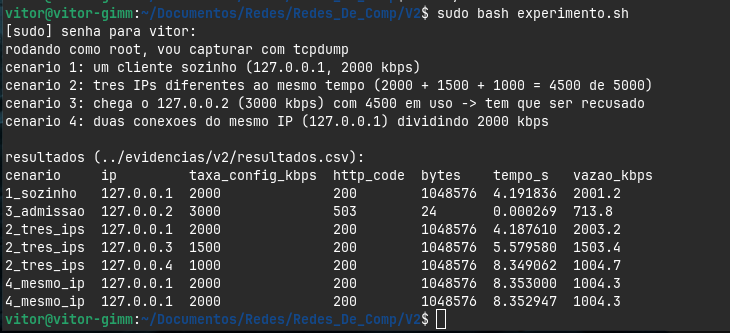
\includegraphics[width=0.92\linewidth]{Captura de tela de 2026-10-17 18-19-01.png}
\caption{Saída do script de experimento executado com captura de pacotes.}
\label{fig:print}
\end{figure}

\begin{table}[h]
\centering
\caption{Vazão útil observada por cenário (objeto de 1\,MiB).}
\label{tab:res}
\small
\begin{tabular}{@{}llrrrr@{}}
\toprule
\textbf{Cenário} & \textbf{IP} & \textbf{Taxa (kbps)} & \textbf{Status} & \textbf{Tempo (s)} & \textbf{Vazão (kbps)} \\
\midrule
1 -- isolado      & 127.0.0.1 & 2000 & 200 & 4,192 & 2001,2 \\
2 -- três IPs     & 127.0.0.1 & 2000 & 200 & 4,188 & 2003,2 \\
2 -- três IPs     & 127.0.0.3 & 1500 & 200 & 5,580 & 1503,4 \\
2 -- três IPs     & 127.0.0.4 & 1000 (padrão) & 200 & 8,349 & 1004,7 \\
3 -- admissão     & 127.0.0.2 & 3000 & 503 & --- & --- \\
4 -- mesmo IP     & 127.0.0.1 & 2000 / 2 & 200 & 8,353 & 1004,3 \\
4 -- mesmo IP     & 127.0.0.1 & 2000 / 2 & 200 & 8,353 & 1004,3 \\
\bottomrule
\end{tabular}
\end{table}

Em todos os cenários aceitos, a vazão ficou no máximo 0,5\% acima da taxa configurada.
A pequena diferença para cima ocorre porque a espera após o último bloco não atrasa o
cliente, que já recebeu todos os dados.
No cenário~2, cada IP recebeu sua própria taxa, inclusive o endereço não cadastrado, que
foi atendido a 1000\,kbps. No cenário~3, com 4500\,kbps em uso, a admissão de mais
3000\,kbps excederia os 5000\,kbps; o servidor respondeu 503 às duas conexões abertas pelo
curl (uma para cada URL), e o registro indicou \texttt{RECUSADO ip=127.0.0.2}. No
cenário~4, as duas conexões de 127.0.0.1 levaram praticamente o dobro do tempo do
cenário~1, com cerca de 1000\,kbps cada, confirmando a divisão da taxa. O HTML de 532 bytes
foi entregue em menos de 1\,ms em todos os casos.

A Figura~\ref{fig:painel} reproduz o painel registrado durante os cenários~2 e~4.

\begin{figure}[h]
\centering
\scriptsize
\begin{verbatim}
vazao usada: 4500 / 5000 kbps   conexoes ativas: 3
IP          CON  TAXA_IP  TAXA/CON  RTT(ms)  ATRASO(ms)  BANDA(kbps)  REAL(kbps)  ENVIADO
127.0.0.3     1     1500      1500      1.0         0.5       4256.0      1515.8    512KB
127.0.0.4     1     1000      1000      1.0         0.5       4256.0      1021.0    344KB
127.0.0.1     1     2000      2000      1.0         0.5       4256.0      2011.8    680KB

vazao usada: 2000 / 5000 kbps   conexoes ativas: 2
IP          CON  TAXA_IP  TAXA/CON  RTT(ms)  ATRASO(ms)  BANDA(kbps)  REAL(kbps)  ENVIADO
127.0.0.1     2     2000      1000      1.0         0.5       4256.0      1022.7   1632KB
\end{verbatim}
\caption{Painel do servidor durante os cenários 2 (acima) e 4 (abaixo).}
\label{fig:painel}
\end{figure}

\subsection{Análise da captura de pacotes}

A captura do experimento (\texttt{experimento.pcap}) contém 1647 pacotes em 8 conexões
TCP, todas com \emph{handshake} completo (8 SYN e 8 SYN-ACK). Foram observadas 14
requisições GET e 12 respostas 200: seis clientes admitidos com duas requisições cada e
duas conexões recusadas de 127.0.0.2. Cada cliente admitido usou uma única conexão para o
HTML e o objeto, confirmando a persistência HTTP/1.1.

A Tabela~\ref{tab:pcap} apresenta, por conexão, o intervalo mediano entre segmentos de
dados do objeto. Como a MTU do \emph{loopback} é de 64\,KiB, cada bloco de 8\,KiB foi
transmitido em um único segmento, o que torna visível o ritmo imposto pelo servidor. O
intervalo teórico é $8 \times 8192 / R_c$ ms.

\begin{table}[h]
\centering
\caption{Intervalo entre segmentos de 8\,KiB obtido da captura.}
\label{tab:pcap}
\small
\begin{tabular}{@{}lrrrr@{}}
\toprule
\textbf{Conexão} & \textbf{Taxa/conexão (kbps)} & \textbf{Teórico (ms)} & \textbf{Medido (ms)} & \textbf{Vazão na captura (kbps)} \\
\midrule
127.0.0.1 (cen. 1) & 2000 & 32,77 & 33,03 & 2001,4 \\
127.0.0.3 (cen. 2) & 1500 & 43,69 & 43,95 & 1503,6 \\
127.0.0.4 (cen. 2) & 1000 & 65,54 & 65,76 & 1004,9 \\
127.0.0.1 (cen. 4) & 1000 & 65,54 & 65,79 & 1004,4 \\
\bottomrule
\end{tabular}
\end{table}

O intervalo medido é cerca de 0,25\,ms maior que o teórico em todos os casos. Essa
diferença corresponde ao tempo de leitura do arquivo e de envio do bloco, que não é
descontado da espera. No \emph{loopback}, o efeito é pequeno; em redes com envio mais lento,
a vazão obtida tenderá a ficar abaixo da configurada.

\subsection{Discussão e limitações}

No \emph{loopback}, o intervalo entre a requisição do HTML e a do objeto observado na
captura foi de 0,29 a 0,44\,ms. Como o servidor mede em milissegundos e aplica mínimo de
1\,ms, o painel exibiu RTT de 1,0\,ms e banda estimada de 4256\,kbps ($532 \times 8 / 1$)
para todos os clientes. Esses valores refletem a resolução da medição, e não a capacidade
real do enlace. Além disso, o intervalo inclui o tempo de transmissão do HTML e de
processamento do cliente, de modo que não deve ser interpretado como medição direta do
atraso unidirecional.

Outras limitações conhecidas são: a divisão inteira da taxa entre conexões; o arquivo de
taxas não aceitar comentários; e a coluna de bytes enviados do painel ser acumulada
enquanto o registro do IP for mantido. Os experimentos em rede cabeada (IEEE 802.3) e sem
fio (IEEE 802.11), com hosts distintos, e as medições com IPTraf ainda não foram
realizados. Eles estão previstos para a validação com o docente, quando as estimativas de
RTT e banda poderão ser avaliadas em condições reais.

%=====================================================================
\section{Conclusões}

A segunda versão incorporou os mecanismos de QoS previstos: taxa por IP com valor padrão,
controle de envio para objetos não HTML, divisão da taxa entre conexões do mesmo IP,
controle de admissão pela vazão máxima e painel em tempo real. Os experimentos confirmaram
que as vazões obtidas acompanharam as taxas configuradas, que a divisão entre conexões
ocorreu como esperado e que um cliente acima da capacidade foi recusado. A captura de
pacotes mostrou que o espaçamento dos segmentos TCP segue a taxa definida pelo servidor.

Como próximos passos, a equipe pretende: repetir os experimentos em Ethernet e Wi-Fi com
hosts distintos, utilizando IPTraf e Wireshark; aumentar a resolução da medição do RTT;
descontar o tempo de envio no cálculo da espera; e preparar a demonstração para o docente
até 26/10.

\section{Uso de ferramentas de IA}

Conforme exigido pelo enunciado, parte do código da segunda versão e dos scripts de teste
foi produzida com apoio de IA (Claude, da Anthropic) e revisada pela equipe. Esse uso está
indicado no início de \texttt{V2/src/server.c} e no \texttt{V2/README.md}.

\section{GitHub}

Código-fonte, scripts e evidências:
\url{https://github.com/giovanapiazza/Redes_De_Comp} (pastas \texttt{V2} e
\texttt{evidencias/v2}).

\begin{thebibliography}{9}
\bibitem{spec} Fundamentos e Avaliação de Redes de Computadores (2026). Trabalho de
programação em rede: especificação do trabalho prático. Ano letivo/semestre 2026/2.
\bibitem{forouzan} Forouzan, B. A.; Mosharraf, F. (2013). \emph{Redes de computadores: uma
abordagem top-down}. Porto Alegre: AMGH.
\bibitem{rfc9112} Fielding, R.; Nottingham, M.; Reschke, J. (2022). HTTP/1.1. RFC 9112.
IETF. \url{https://www.rfc-editor.org/rfc/rfc9112}.
\bibitem{rfc9110} Fielding, R.; Nottingham, M.; Reschke, J. (2022). HTTP Semantics.
RFC 9110. IETF. \url{https://www.rfc-editor.org/rfc/rfc9110}.
\bibitem{llnl} Lawrence Livermore National Laboratory. POSIX Threads Programming.
\url{https://computing.llnl.gov/tutorials/pthreads/}.
\end{thebibliography}

\end{document}
